\section{External Fields}
Up to this point, we have discussed the fine and hyperfine structure, and discussed what the real spectrum of the hydrogen atom looks like.

\begin{figure}[htbp]
    \centering
    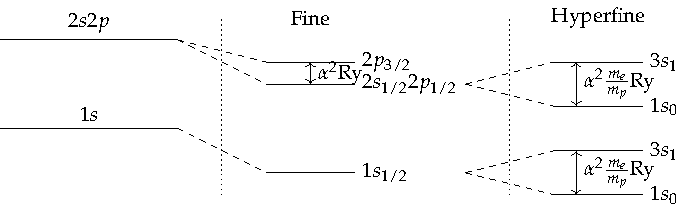
\includegraphics[]{Images/fig-hyperfinestructuresplit.pdf}

    \caption{Splitting in hydrogen atom energy levels due to the fine structure and hyperfine structure. Figure is not to scale (the hyperfine splittings are $\sim 10^{-3}$ smaller compared to the fine structure). Note the hyperfine splitting only occurs for the $s$ states (as it only occurs for states whose radial wavefunction is nonvanishing at the origin) and the split is between the singlet and triplet states. The $3/1$ denotes triplet/singlet and the $1/0$ denotes the total joint spin as $1$ or $0$.}
    \label{fig-hyperfinestructuresplit}
\end{figure}

However note that thus far we have only discussed internal fields. We today discuss external ones.

\subsection{Stark Effect - Large Field}
We consider a hydrogen atom in the presence of an electric field (in particular oriented in the $z$ direction). This has the corresponding Hamiltonian:
\begin{equation}
    H^{(1)} = -\v{d} \cdot \v{E}^{ext} = -ezE_z^{ext}
\end{equation}
We now ask what the typical scale of this perturbation is. $z \sim a_B$, so it is of scale $e a_B E_{ext}$. We consider the limit where the external field is much stronger than the fine structure corrections:
\begin{equation}
    e a_B E^{ext} \gg \alpha^2 \si{Ry} \sim 10^{-5} 10 \si{eV}
\end{equation}
and so:
\begin{equation}
    E^{ext} \gg \frac{ 10^{-5} 10 \si{eV}}{\abs{e}10^{-8}\si{m}} \sim 10^{4}\si{V.cm^{-1}}.
\end{equation}

Are fields of such magnitude present in nature? Certainly; consider a thunderstorm. Lab-wise, the largest field we can achieve is $100\si{MeV.m^{-1}}$, or $10^{6}\si{V.cm^{-1}}$ in linear accelerators. We discuss this large field limit, so we can do perturbation theory not with the fine structure states but with the unperturbed hydrogen atom states $\ket{n, l}$. We consider:
\begin{equation}
    \bra{n=1, l=0}H^{(1)}\ket{n=1,l=0} = 0
\end{equation}
This can be seen from the fact that $H' \propto z$, and then using that $\ket{n=1, l=0}$ are eigenstates of parity (with eigenvalue $1$), by symmetry we see that:
\begin{equation}\label{eq-paritymatelezero}
    \begin{split}
        \bra{n=1, l=0}H^{(1)}\ket{n=1, l=0} &\propto \bra{n=1, l=0}z\ket{n=1, l=0} 
        \\ &= \bra{n=1, l=0}\Pi^\dag z \Pi \ket{n=1, l=0} 
        \\ &= \bra{n=1, l=0}(-1)z \ket{n=1, l=0} 
        \\ &= -\bra{n=1, l=0}z\ket{n=1, l=0}
    \end{split}
\end{equation}
and so the matrix element must vanish. In calculating the energy correction, we have degeneracy and thus must use degenerate PT. To this end it is useful to consider what the good quantum numbers are. First, we see that:
\begin{equation}
    [L_z, H^{(1)}] = 0
\end{equation}
as $H^{(1)} \propto z$. However:
\begin{equation}
    [\v{L}^2, H^{(1)}] \neq 0
\end{equation}
as we do not have a general rotational symmetry here, only a symmetry for rotations about $z$.

In particular, let us consider the $n = 2$ states of hydrogen There are four degenerate states:
\begin{itemize}
    \item $\ket{n=2, l=0, m=0}$
    \item $\ket{n=2, l=1, m=0}$
    \item $\ket{n=2, l=1, m=1}$
    \item $\ket{n=2, l=1, m=-1}$
\end{itemize}
We now consider the matrix $T_{ab}$ of matrix elements of $H^{(1)}$ with the above states. But we find that all but two numbers vanish:
\begin{equation}
    T_{ab} = \m{0 & \cdot & 0 & 0 \\ \cdot & 0 & 0 & 0 \\ 0 & 0 & 0 & 0 \\ 0 & 0 & 0 & 0}
\end{equation}
and in particular we only need to compute one by Hermicity. How to see this? First, since $m$ is a good quantum number, only matrix elements with the same $m$ are nonzero. Second, only eigenstates of different parities will have a nonzero matrix element; else we could repeat the argument in Eq. \eqref{eq-paritymatelezero} to conclude that these matrix elements vanish. In other words, only matrix elements with the same $m$ and $l$s of different parity (actually more specifically $\delta l = \pm 1$) will be nonvanishing. Therefore the only matrix element to compute is:
\begin{equation}
    \begin{split}
        T_{12} &= \bra{n=2, l=1, m=0}-erE\cos\theta \ket{n=2, l=0, m=0}
        \\ &= -e\int R_{20} r R_{21} r^2 dr \int Y^0_0 \cos\theta Y_1^1 d\Omega
        \\ &= 3eaE^{ext}
    \end{split}
\end{equation}
so:
\begin{equation}
    T_{ab} = 3eaE^{ext}\m{0 & 1 & 0 & 0 \\ 1 & 0 & 0 & 0 \\ 0 & 0 & 0 & 0 \\ 0 & 0 & 0 & 0}
\end{equation}
So our computation reduces to:
\begin{equation}
    \det(T_{ab} - \delta_{ab}E^{(1)}) = \det\m{-E^{(1)} & 3eaE \\ 3eaE & -E^{(1)}} = 0
\end{equation}
we hence obtain:
\begin{equation}
    E^{(1)}_\pm = \pm 3eaE
\end{equation}
These have corresponding eigenvectors:
\begin{equation}
    \v{v}_+ = \frac{1}{\sqrt{2}}\m{1\\1}, \quad \v{v}_- = \frac{1}{\sqrt{2}}\m{1\\-1}
\end{equation}
So therefore the superpositions of interest are:
\begin{equation}
    \psi_\pm = \frac{1}{\sqrt{2}}\left(\ket{n=2, l=1, m=0} \pm \ket{n=2, l=0, m=0}\right)
\end{equation}
with energies:
\begin{equation}
    E = E_0 \pm E^{(1)} =  -\frac{1}{4}\si{Ry} \pm 3eaE 
\end{equation}
Graphically, we have the spectrum:
\begin{figure}[htbp]
    \centering
    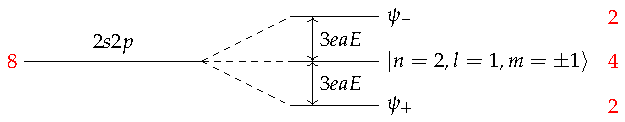
\includegraphics[]{Images/fig-strongstarkeffectsplit.pdf}
    
    \caption{(Linear) Stark Effect splitting of the 8-fold degenerate $2s2p$ energy level in the Hydrogen atom in the presence of a strong external electric field. The energy level splits into three levels, separated by $3eaE$. The degeneracies of the new levels are denoted in red.}
    \label{fig-strongstarkeffectsplit}
\end{figure}

We still have the degeneracy from the spin (although it does not factor into the problem here), and one of the levels remains without a change in the energy. Note that if we included fine structure on top of this, we would have a further splitting in the above diagram (but of a much smaller order of magnitude than the E-field splitting). Note also that if the electric field perturbation was on the same order of magnitude as the fine structure perturbation, then we would consider the perturbing Hamiltonian to be the sum of the E-field and fine structure terms, and we would have to diagonalize a much less simple $T_{ab}$ matrix.

\subsection{Stark Effect - Small Field}
We now consider an electric field that is small on the scale of the fine structure corrections. We apply the perturbations onto the fine structure corrected states. The $1s_{1/2}$ state remains unaffected (there is no correction from the electric field here, independent of the field strength - all states have the same parity of $l = 0$ here so there cannot be any correction).

There is also no splitting for the $2p_{3/2}$ as all of the matrix elements would be zero. Again, the same parity argument; all four states here have $l = 1$ and so the matrix elements vanish.

The only level which exhibits splitting is the $2s_{1/2}2p_{1/2}$ level as there can be nonzero matrix elements between the $l = 1$ and $l = 0$ states. In particular we obtain (without going through the entire calculation again):
\begin{equation}
    \ket{\psi_\pm} = \frac{1}{\sqrt{2}}\left(\ket{l=1, m=0, s_z = \frac{1}{2}} \pm \ket{l=1, m=1, s_z = -\frac{1}{2}}\right)
\end{equation}
(Ok, this was not so clear to me here how the above formula follows, but oh well). The energy splitting can be seen in Fig.

\begin{figure}[htbp]
    \centering
    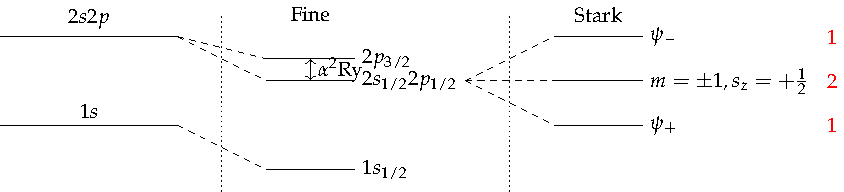
\includegraphics[]{Images/fig-weakstarkeffectsplit.pdf}
    
    \caption{Stark effect splitting of the $2s_{1/2}2p_{1/2}$ (fine structure) energy level due to a weak external electric field. The fourfold degenerate level splits into three levels.}
    \label{fig-weakstarkeffectsplit}
\end{figure}

\subsection{Selection Rules - Calculating expectation values of z}
Let us consider a general matrix element:
\begin{equation}
    \bra{n'l'm'}z\ket{nlm}
\end{equation}
Since $[L_z, z] = 0$, we have:
\begin{equation}
    \bra{n'l'm'}L_z z - zL_z\ket{nlm} = 0 \implies (m' - m)\bra{l'm'}z\ket{lm} = 0
\end{equation}
and so if $m \neq m'$ then the matrix element must vanish. So we obtain the selection rule that $m = m'$. 

Now, we consider the selection rule based on $l$. We will find that $\Delta l = \pm 1$ must be enforced for the matrix element must be zero (the parity argument we make previously only establishes that the $l$s must be of different parity; this is a stronger condition). There is an argument from Clebsch-Gordon coefficients that can show this condition to be true.

\subsection{Zeeman Effect}
We consider an external magnetic field, giving rise to a perturbing Hamiltonian:
\begin{equation}
    H^{(1)} = -\gv{\mu} \cdot \v{B}^{ext}, \quad \gv{\mu}\frac{-\abs{e}\hbar}{2mc}\left(\v{L} + 2\v{S}\right)
\end{equation}
Numerically:
\begin{equation}
    \frac{\abs{e}\hbar}{2mc} = 5.8 \times 10^{-9}\si{eVG^{-1}}
\end{equation}
(we igonore the proton; its contribution is supressed by 2000 or so). We have a strong Zeeman effect when:
\begin{equation}
    \mu B^{ext} \gg \alpha^2 \si{Ry}
\end{equation}
or when:
\begin{equation}
    B^{ext} \gg \frac{10^{-5}10\si{eV}}{10 10^{-9} \si{eV}} G = 10^4 \si{G} = 1\si{T}
\end{equation}
so if the external B-field is much larger than a Tesla, then we have a strong-field Zeeman effect (and weak-field Zeeman effect if much less than a Tesla). 

For scales, MRI/NMR is on the order of Tesla, the LHC is on the order of 10 Tesla, and Earth's B-field is on the order of half a Gauss.

Looking at the commutation relations, we have:
\begin{equation}
    [H', \v{L}^2] = [H', L_z] = [H', \v{S}^2] = [H', \v{S}^2] = 0
\end{equation}
as is clear from looking at the Hamiltonian. We can do the whole matrix elements, and it will be a simple matter of:
\begin{equation}
    \Delta E = \bra{\cdot}2S_z + L_z\ket{*} \frac{-\abs{e}\hbar}{2mc}
\end{equation}
and this is trivial as of course the states are eigenstates of $L^2, S^2, L_z, S_z$! The energy splitting from the (strong-field) Zeeman effect therefore looks as in Fig. 

\begin{figure}[htbp]
    \centering
    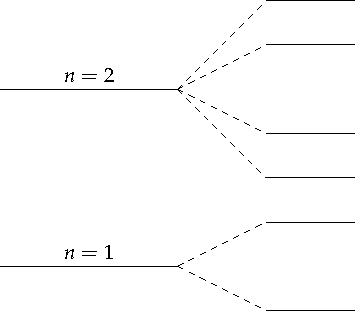
\includegraphics[]{Images/fig-strongzeemaneffectsplit.pdf}

    \caption{Energy splitting of the hydrogen atom levels from the strong-field Zeeman effect.}
    \label{fig-strongzeemaneffectsplit}
\end{figure}

This correction becomes less trivial when the magnetic field is weaker (as we need to take into account the fine structure... and so our states we use are no longer eigenstates of $L^2, S^2, L_z, S_z$); but we can still do the calculation of the matrix elements above. It will be convenient to write it as $\bra{\cdot}J_z + S_z\ket{\cdot}$ instead.

The last question of the HW asks for considerin the interplay of fine hyperfine, and zeeman effects in the Hydrogen atom; have fun! We start WKB next week.